\documentclass[border=4pt]{standalone}
\usepackage{amsmath,amssymb,amsfonts}
\usepackage{xcolor,colortbl,array,booktabs,multirow}
\usepackage{tikz}
\usepackage{pgfplots}
\pgfplotsset{compat=1.16}
\usetikzlibrary{arrows, automata, backgrounds, calendar, chains, decorations,
    matrix, mindmap, patterns, petri, positioning, shadows, shapes.geometric,
    trees, shapes, decorations.pathreplacing, calc, tikzmark, arrows.meta,
    intersections, fit, graphs, quotes, angles, decorations.markings}
\newcommand{\st}{\text{ s.t. }}
\newcommand{\x}{\mathbf{x}}
\renewcommand{\b}{\mathbf{b}}
\renewcommand{\c}{\mathbf{c}}
\newcommand{\A}{\mathbf{A}}
\newcommand{\y}{\mathbf{y}}
\newcommand{\z}{\mathbf{z}}
\newcommand{\R}{\mathbb{R}}
\newcommand{\RR}{\mathbb{R}}
\newcommand{\Z}{\mathbb{Z}}
\newcommand{\ZZ}{\mathbb{Z}}
\newcommand{\npcomplete}{NP-complete}
\providecommand{\true}{\text{TRUE}}
\providecommand{\false}{\text{FALSE}}
\tikzset{vertex/.style={circle,fill=black!25,minimum size=20pt,inner sep=0pt},
    edge/.style={draw,thick,-},weight/.style={font=\small},
    selected vertex/.style={vertex, fill=red!24},
    selected edge/.style={draw,line width=2pt,-,red!50},
    ignored edge/.style={draw,line width=2pt,-,black!20}}
\newcommand{\vect}{\vec}
\providecommand{\ds}{\displaystyle}
\providecommand{\longvect}{\overrightarrow}
\usepackage[normalem]{ulem}
\definecolor{ocre}{RGB}{243,102,25}
\providecommand{\leftB}{\left[}
\providecommand{\rightB}{\right]}
\tikzset{directed/.style={postaction={decorate,decoration={markings,mark=at position .65 with {\arrow{>}}}}},
    directed1/.style={postaction={decorate,decoration={markings,mark=at position .65 with {\arrow{>}}}}}}
\begin{document}
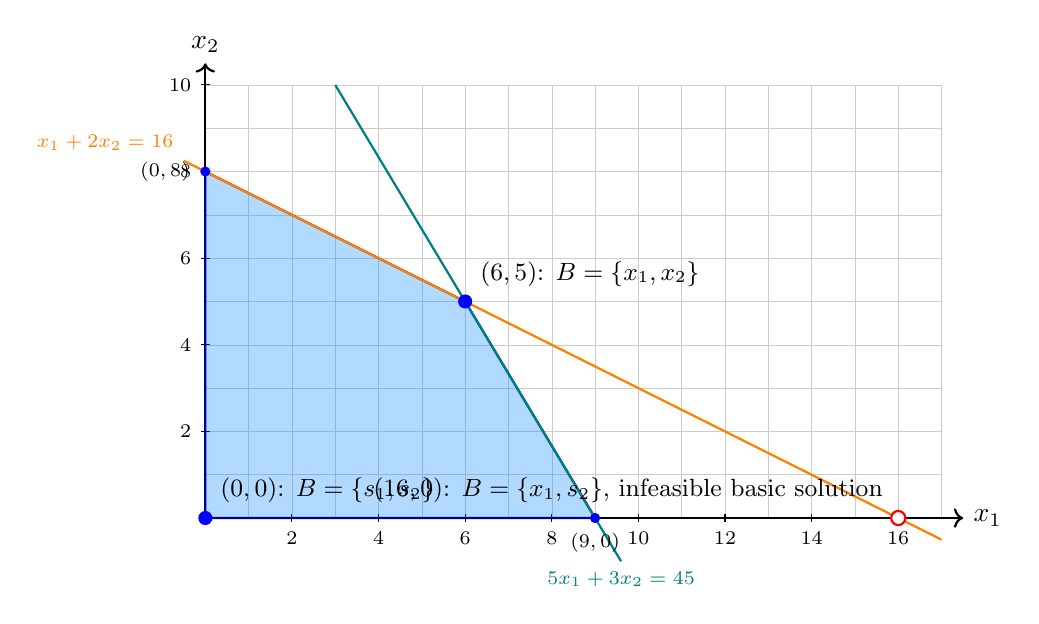
\begin{tikzpicture}[scale=0.55]
    % Grid and axes
    \draw[gray!40, very thin, step=1] (0,0) grid (17,10);
    \draw[->, thick] (0,0) -- (17.5,0) node[right] {$x_1$};
    \draw[->, thick] (0,0) -- (0,10.5) node[above] {$x_2$};
    \foreach \x in {2,4,...,16} \draw (\x,0.1) -- (\x,-0.1) node[below] {\scriptsize \x};
    \foreach \y in {2,4,...,10} \draw (0.1,\y) -- (-0.1,\y) node[left] {\scriptsize \y};

    % Feasible region
    \fill[blue!50!cyan, opacity=0.3] (0,0) -- (9,0) -- (6,5) -- (0,8) -- cycle;
    \draw[blue!60!black, thick] (0,0) -- (9,0) -- (6,5) -- (0,8) -- cycle;

    % Constraint boundaries
    \draw[orange, thick] (-0.5,8.25) node[above left] {\scriptsize $x_1+2x_2=16$} -- (17,-0.5);
    \draw[teal, thick] (3,10) -- (9.6,-1) node[below] {\scriptsize $5x_1+3x_2=45$};

    % Remaining vertices of the region
    \node[fill=blue,circle,inner sep=1.3pt,label={below:\scriptsize $(9,0)$}] at (9,0) {};
    \node[fill=blue,circle,inner sep=1.3pt,label={left:\scriptsize $(0,8)$}] at (0,8) {};

    % Basic solutions from the three bases
    \node[fill=blue,circle,inner sep=1.8pt,
        label={above right:\small $(6,5)$: $B=\{x_1,x_2\}$}] at (6,5) {};
    \node[fill=blue,circle,inner sep=1.8pt,
        label={above right:\small $(0,0)$: $B=\{s_1,s_2\}$}] at (0,0) {};
    \node[draw=red,thick,circle,fill=white,inner sep=1.8pt,
        label={above left:\small $(16,0)$: $B=\{x_1,s_2\}$, infeasible basic solution}] at (16,0) {};
\end{tikzpicture}
\end{document}
